\definecolor{light}{cmyk}{0.2,0.2,0.2,0}
\definecolor{dark}{cmyk}{0.8,0.8,0.8,0.0}

\tikzstyle{peers}=[draw,circle, bottom color=dark, minimum width=10pt]
\tikzstyle{superpeers}=[draw,rectangle, rounded corners, bottom color=light, minimum width=20pt, minimum height = 20pt]

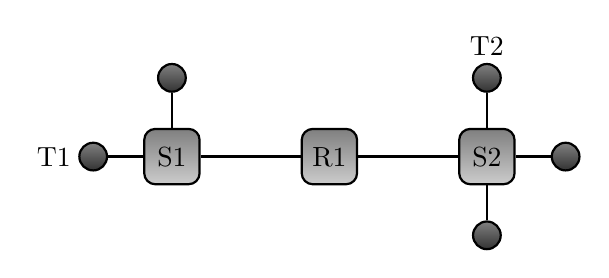
\begin{tikzpicture}[auto, thick]
  \node[peers] (T1) at (2,3) {};
  \node[peers] (T2) at (1,2) {};
  \node[superpeers] (S1) at (2,2) {S1};
  \path (T1) edge (S1);
  \path (T2) edge (S1);
  
  \node[superpeers] (R1) at (4,2) {R1};
  \path (S1) edge (R1);
  
  \node[superpeers] (S2) at (6,2) {S2};
  \path (R1) edge (S2);
  
  \node[peers] (T3) at (6,3) {};
  \node[peers] (T4) at (7,2) {};
  \node[peers] (T5) at (6,1) {};
  \path (T3) edge (S2);
  \path (T4) edge (S2);
  \path (T5) edge (S2);

  \node (L1) at (0.5,2) {T1};
  \node (L2) at (6,3.4) {T2};
\end{tikzpicture}
